% chap4.tex (Customer Description)

\chapter{Customer Description} 

In this chapter, I will describe the customers present in the PowerTAC simulation system, some statistics about them and their attributes.

\section{Customers}

In PowerTAC simulation system the customers are the entities that buy and sell electricity. A customer subscribes to one of the tariffs published by the brokers and it pays or receives money according to the tariff plan. A customer can represent a population size of one to several thousand. For example, customers that represent an electric vehicle customer represent only one person and the customers that represent a village usually have several thousand populations. In PowerTAC environment there are 168 customers in total.

\section {PowerTypes}
In Power TAC, every customer has a power type. Power type determines the behavior of the customers. A customer that has power type related to production produces electricity. A customer that has a power type related to energy consumption consumes energy. In the following subsections, I describe different power types of the simulation.

\subsection{consumption}

A customer with power type consumption are the most common customers. They use the energy when they need it. They cannot shift their demand to a future timeslot. Usually, they have a regular pattern of their energy usage. Usually, they show a similar pattern for weekdays. They have similar kind of usage pattern for the weekends. 

The figure  \ref{fig:2daysbrook} shows 2 days electricity usage of the BrookSideHomes customer. The pattern shows in a day, around at 10 am there is a growing need for electricity. During the night after 10 pm, the electricity consumption starts decreasing.
\begin{figure}[h!]
  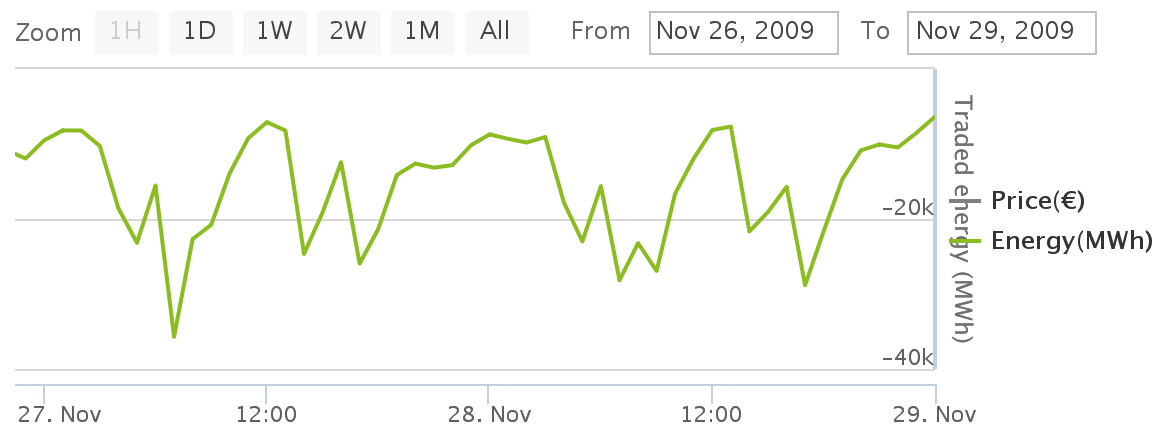
\includegraphics[width=\linewidth]{BrooksideHomes-2days.png}
  \caption{Two days energy usage for the customer Brooksidehomes.}
  \label{fig:2daysbrook}
\end{figure}

The figure \ref{fig:2weekOffice} shows two weeks consumption of the downtown customer. The customer shows a similar pattern for all weekdays. It also shows  distinguishable energy usage during the weekends.

\begin{figure}[h!]
  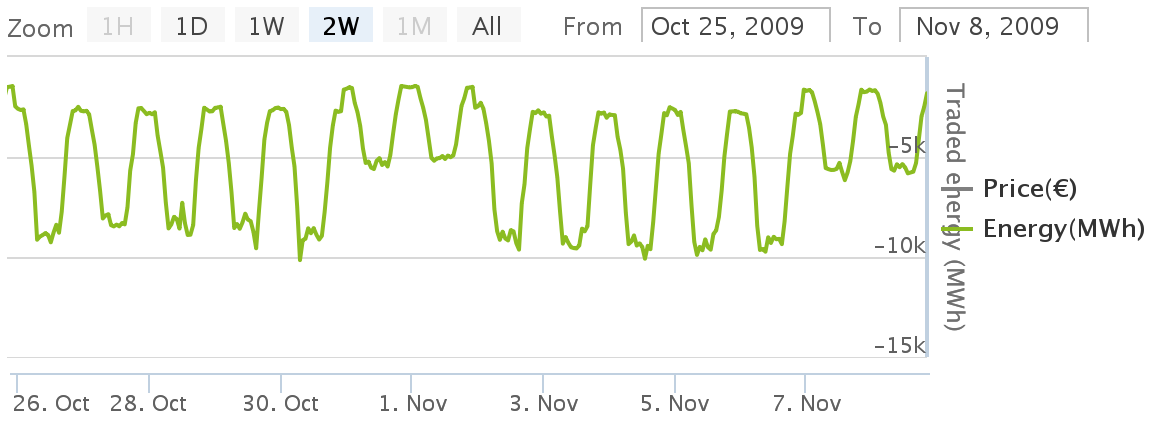
\includegraphics[width=\linewidth]{downtown-offc-2-weeks.png}
  \caption{Two weeks energys usage of the downtown office customer.}
  \label{fig:2weekOffice}
\end{figure}

\subsection{Interruptible Consumption}
Interruptible customers are smart enough to shift their energy demand in a timeslot where they can buy electricity at a reduced price. Because of this shifting capability, they don't show a regular usage pattern as the consumption customers do. Figure \ref{fig:2weekOffice} shows a controllable customer's 2 days usage.

\begin{figure}[h!]
  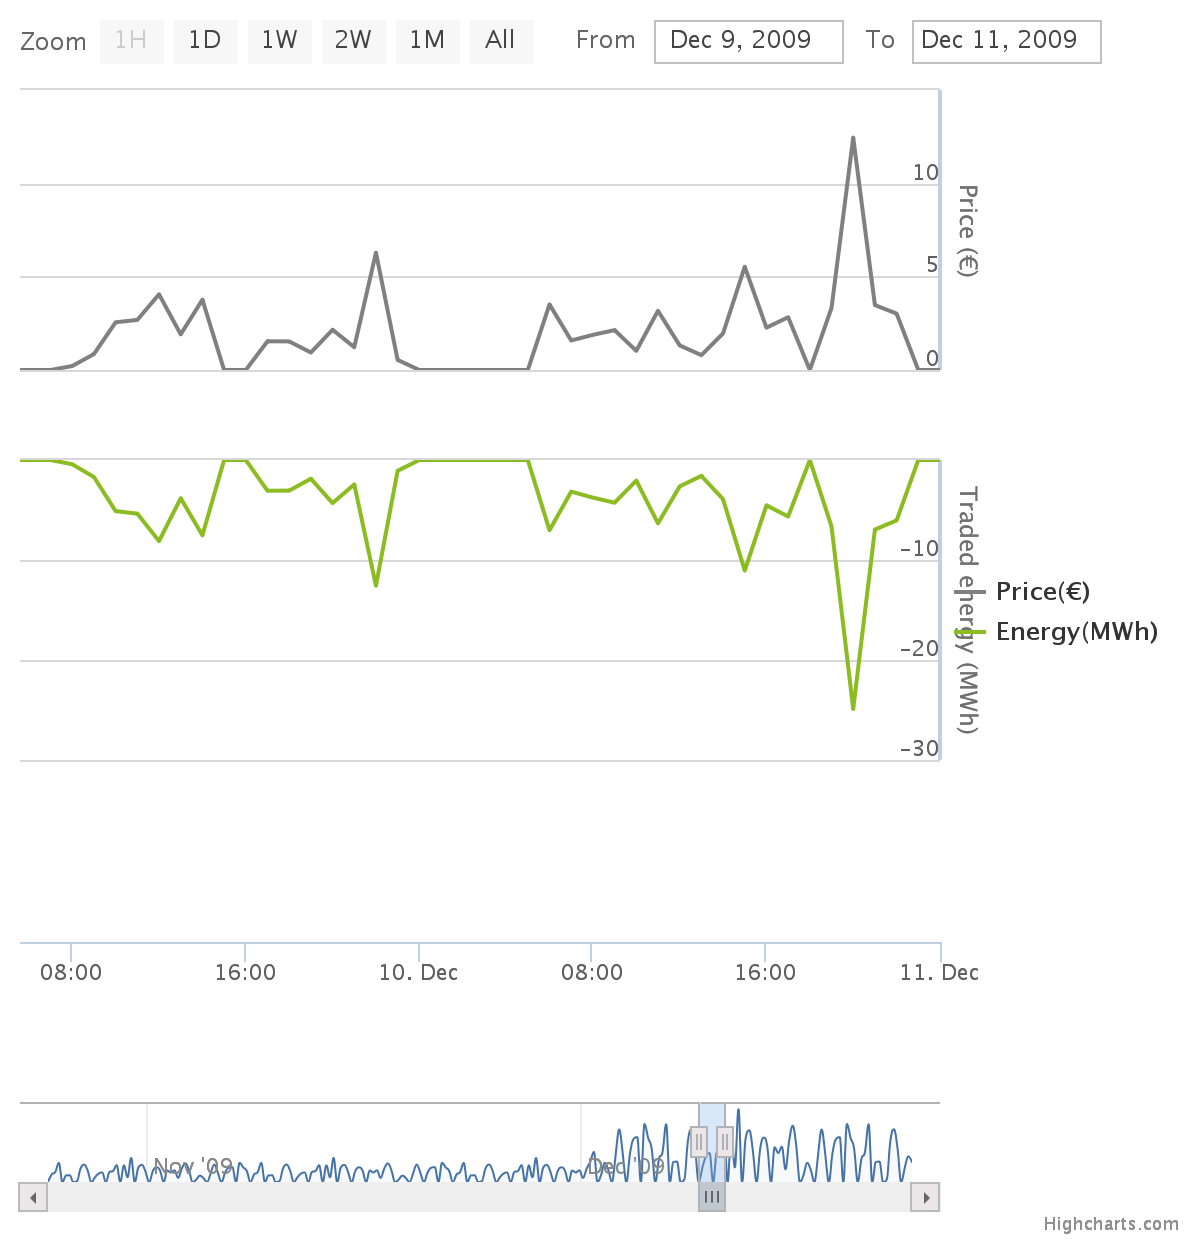
\includegraphics[width=\linewidth]{village2nsControllable.png}
  \caption{Two days energys usage of the village 2 ns controllable customer.}
  \label{fig:2weekOffice}
\end{figure}

\subsection{Thermal Storage}
Thermal storage customers show a weekly pattern in their electricity usage. Also, during a day, their electricity usage in a day depends  much on the energy they used in the last timeslot. Figure \ref{fig:day-thermal} and \ref{fig:thermal-week} shows a day and two week's energy usage of the thermal storage customer sf2.

\begin{figure}[h!]
  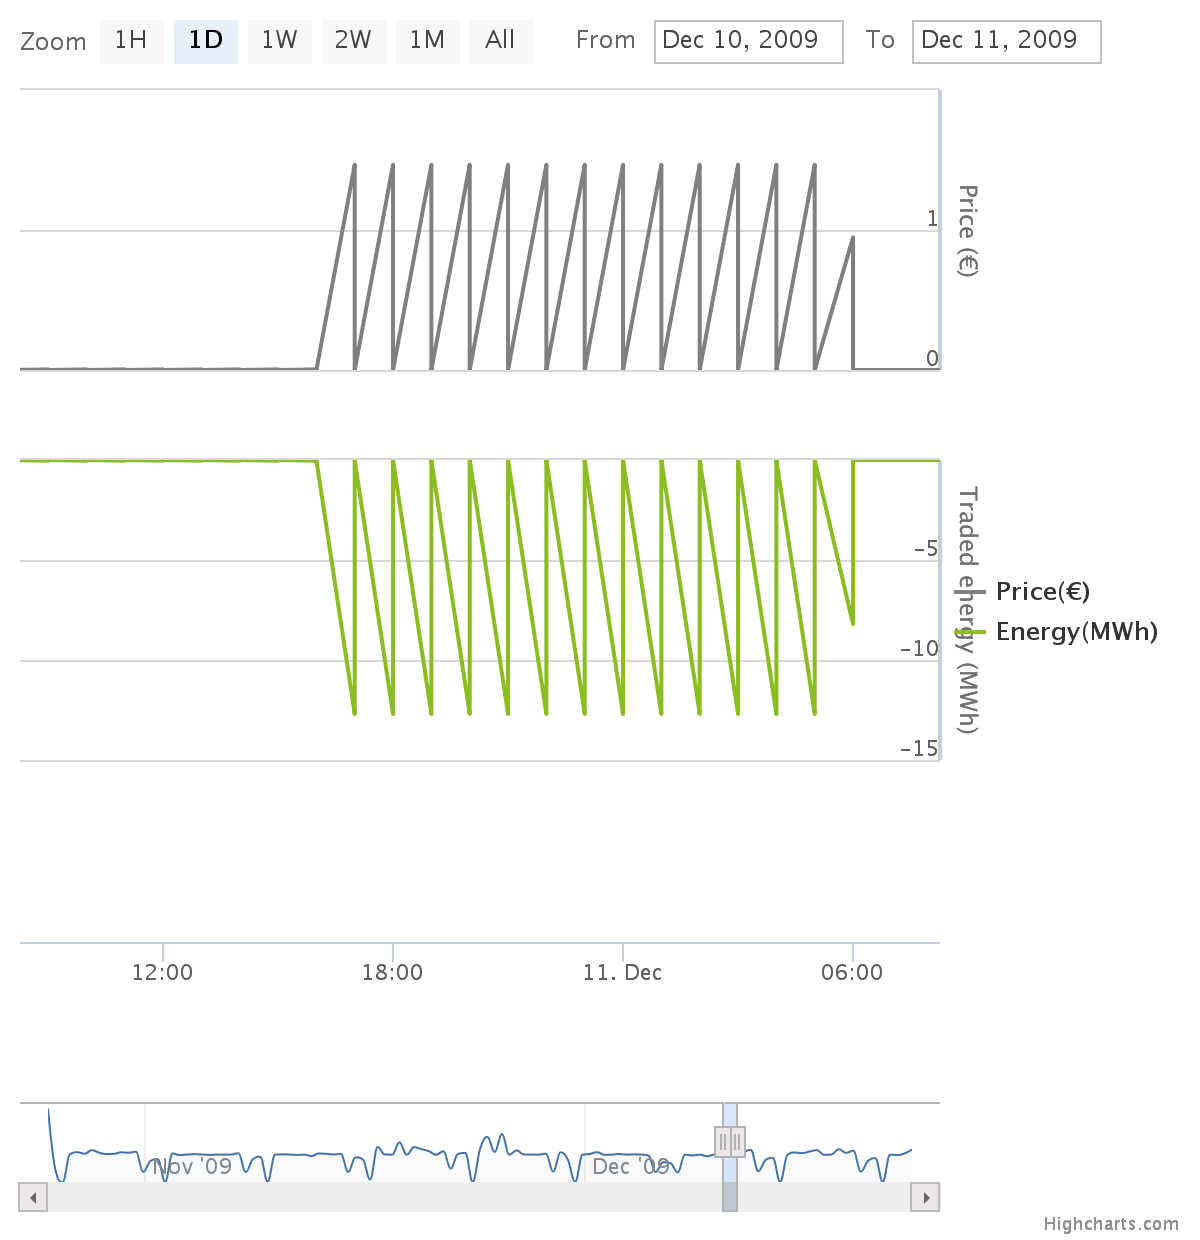
\includegraphics[width=\linewidth]{sf2-thermal-daily.png}
  \caption{A day's energys usage of the sf2 thermal storage customer.}
  \label{fig:day-thermal}
\end{figure}

\begin{figure}[h!]
  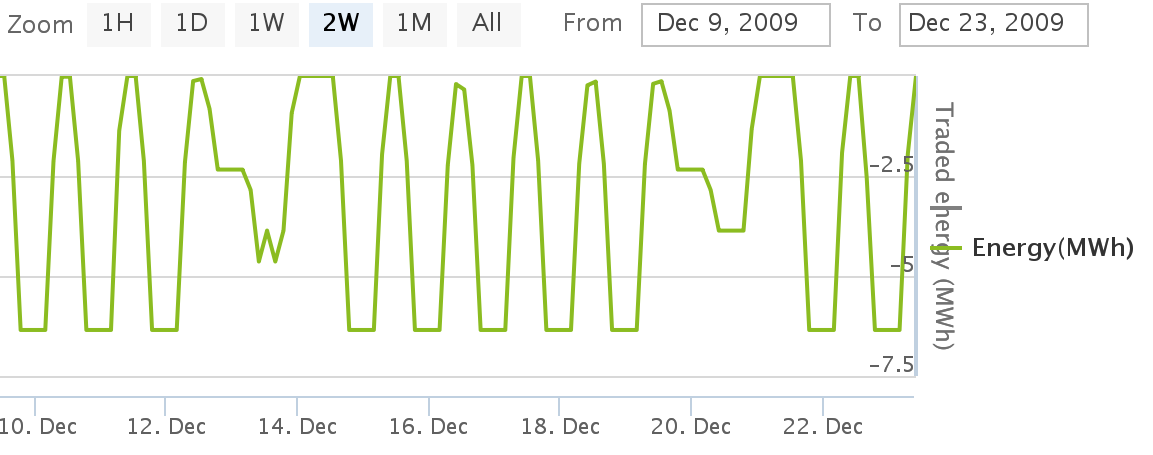
\includegraphics[width=\linewidth]{sf2-thermal-week.png}
  \caption{Two week's energys usage of the sf2 thermal storage customer.}
  \label{fig:thermal-week}
\end{figure}


\subsection{Solar Production}
Figure \ref{fig:solar-twoday} shows two day's and  figure \ref{{fig:solar-oneweek}} shows a week's energy production of the SunnyHill solar production customer. From the figures, we see that during the daytime the solar production customers usually produces electricity which is as expected.

\begin{figure}[h!]
  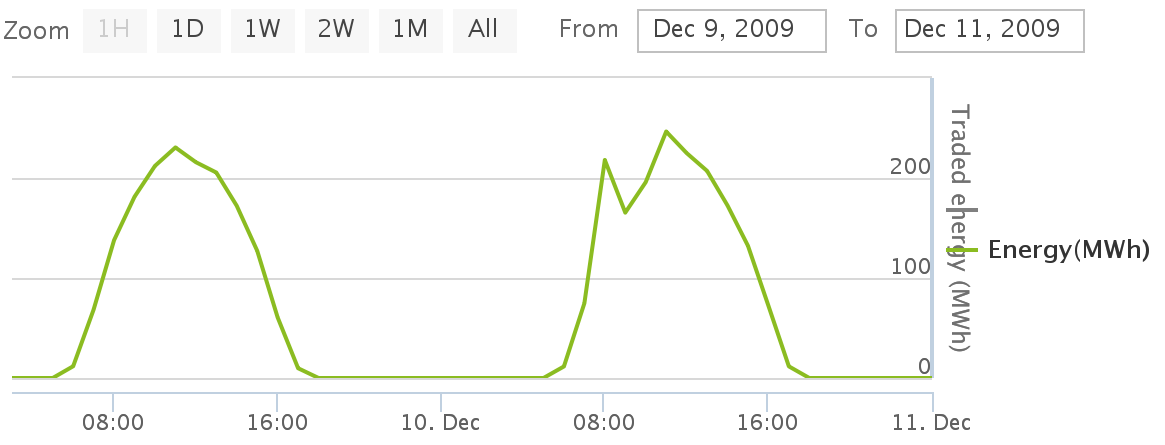
\includegraphics[width=\linewidth]{sunnyhill-twoday.png}
  \caption{Two days energys usage of the SunnyHill solar production.}
  \label{fig:solar-twoday}
\end{figure}


\begin{figure}[h!]
  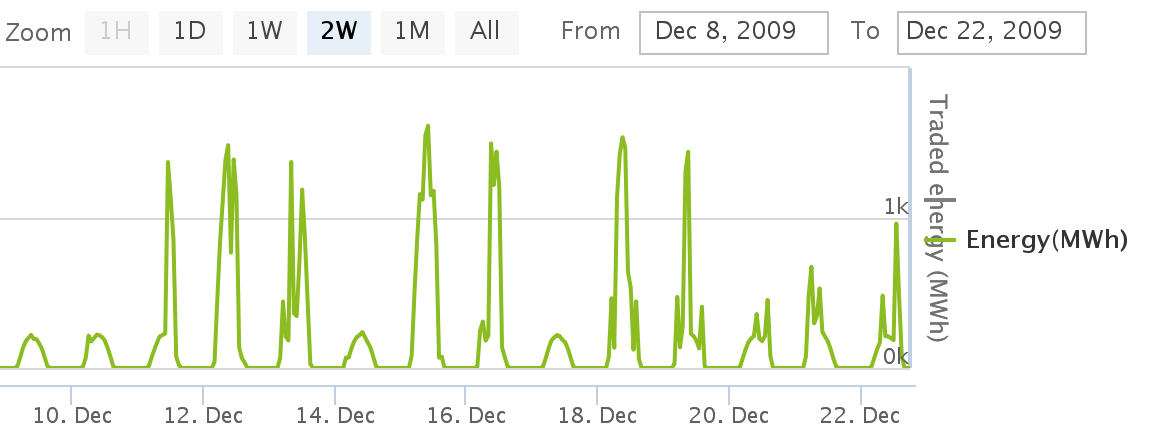
\includegraphics[width=\linewidth]{sunnyhill-oneweek.png}
  \caption{One week's energys usage of the SunnyHill solar production.}
  \label{fig:solar-oneweek}
\end{figure}

\subsection{Wind Production}
Wind production customers generate energy from the wind.
\subsection {Electric Vehicle}
An electric vehicle customer represents one electric vehicle. Their usage of energy is quite irregular and hard to predict.

\section{Statistics}
In this section, I present some statistics on the customers available in the system. 

\subsection {Customer Vs PowerType}

In the figure \ref{fig:cust-pt} we can see the system has more customer with the power type electric vehicle than any other power types. This is because the electric vehicle represents a population of size 1.

\subsection {Population Vs PowerType}
From figure \ref{fig:pop-pt} by far the powertype of consumption has the most number of population.

\subsection {Total Energy Consumed Vs PowerType}
From figure \ref{fig:energy-pt} we can see that the consumption type customers uses the most amount of the electricity.


\begin{figure}
\centering
\begin{minipage}{.5\textwidth}
  \centering
  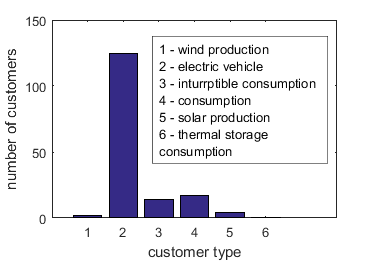
\includegraphics[width=\linewidth]{4-customer-vs-powertype.jpg}
  \caption{Number of customers vs Powertype.}
  \label{fig:cust-pt}
\end{minipage}%
\begin{minipage}{.5\textwidth}
  \centering
  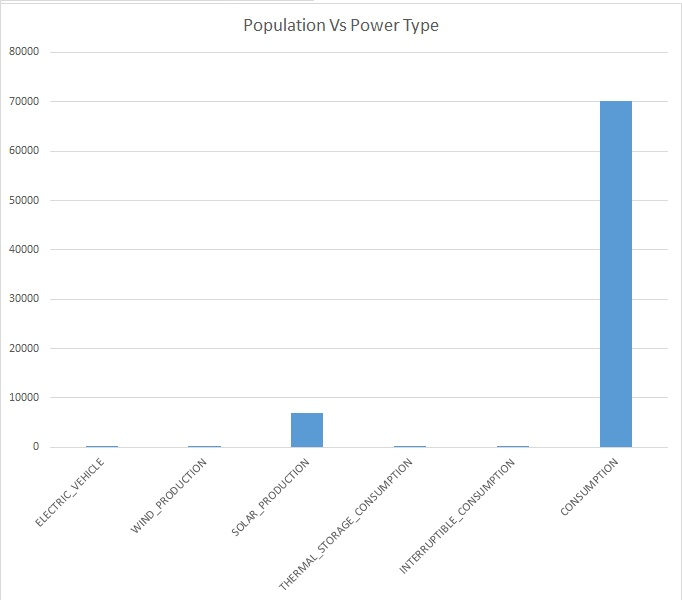
\includegraphics[width=\linewidth]{2-population-vs-powertype.jpg}
  \caption{Population vs Powertype}
  \label{fig:pop-pt}
\end{minipage}

\centering
\begin{minipage}{.5\textwidth}
  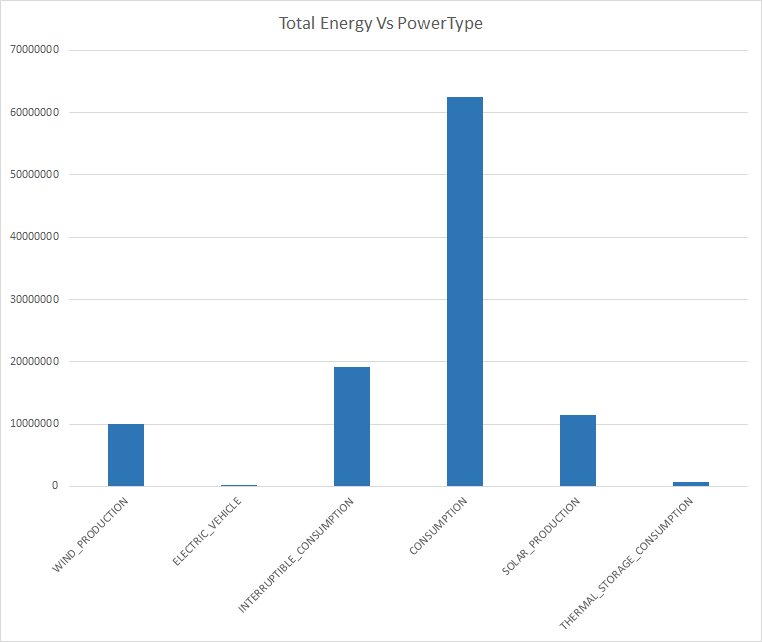
\includegraphics[width=\linewidth]{3-energy-vs-powertype.png}
  \caption{Energy vs PowerType.}
  \label{fig:energy-pt}
\end{minipage}%
\begin{minipage}{.5\textwidth}
  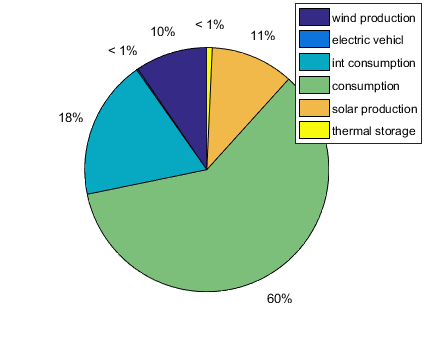
\includegraphics[width=\linewidth]{pie-energy-share.png}
  \caption{Energy share for each power type.}
  \label{fig:energy-shares}
\end{minipage}

\end{figure}